\section{Astronomy Background}\label{sec:ast_terms}
\subsection{The Celestial Sphere}
The celestial sphere is a fundamental concept in astronomy.
It is an imaginary sphere with an arbitrary radius centered on Earth, and it allows us to represent the positions of celestial objects conveniently and intuitively.
Any astronomical observation is a 2D projection onto the celestial sphere,
a tool astronomers use to specify the position of a target as it appears in the sky without using its physical distance from Earth
(which requires a deeper knowledge of the physical properties of the astronomical target, usually acquired after many different observations)
We describe the position as two-dimensional angular coordinates on the sphere.
While the celestial sphere is a universal concept, the coordinate system used to specify the location of a target can vary.




\subsection{Altitude-Azimuth Coordinate System}\label{sec:altaz_coords}
Figure \ref{fig:altaz_coords} depicts the altitude-azimuth coordinate system,
which depends on the observatory's position on Earth and is commonly used when performing astronomical observations
(but rarely used in scientific publications, which instead use a universal coordinate system).
This system specifies the angular coordinates (e.g. in degrees or arcminutes, which are 1/60 of a degree, or arcseconds which are 1/60 of an arcmin)
using an azimuth and an altitude (or elevation) angle.
Azimuth is the angle around the axis perpendicular to the horizontal plane, with zero degrees corresponding to due north.
At APEX, the convention is to increase the azimuth angle in a clockwise direction.
The interval for azimuth angles is $[-270^\circ,270^\circ]$ due to APEX's ability to rotate one and a half times around its axis in the horizontal plane.
On the other hand, elevation is the angle perpendicular to the horizontal plane, with zero degrees corresponding to the telescope pointing at the horizon and $90\degr$ to the telescope pointing at the zenith directly above it.
In this thesis, we used elevation instead of altitude to describe this coordinate.\\


% Another angle term used in this thesis is the horizontal angle.
% We will use the term azimuth when referring to the telescope pointing and the horizontal angle for the pointing offset.
% The azimuth angle is the angle projected on the horizontal plane, while the horizontal angle is the angle measured on the celestial sphere and is dependent on elevation.
% It is essential to know this distinction when measuring offsets and applying its corrections to the pointing model.

% For example, we point at a source at $ Az=El=60\degr $ and observe that the source is $ 1\degr $ to the right.
% The horizontal offset is $1\degr$, while the azimuth offset is $1\degr/\cos{El}=2\degr$.
% Therefore, the azimuth angle must increase by twice the horizontal offset due to the influence of elevation.


\begin{figure}[H]
    \centering
    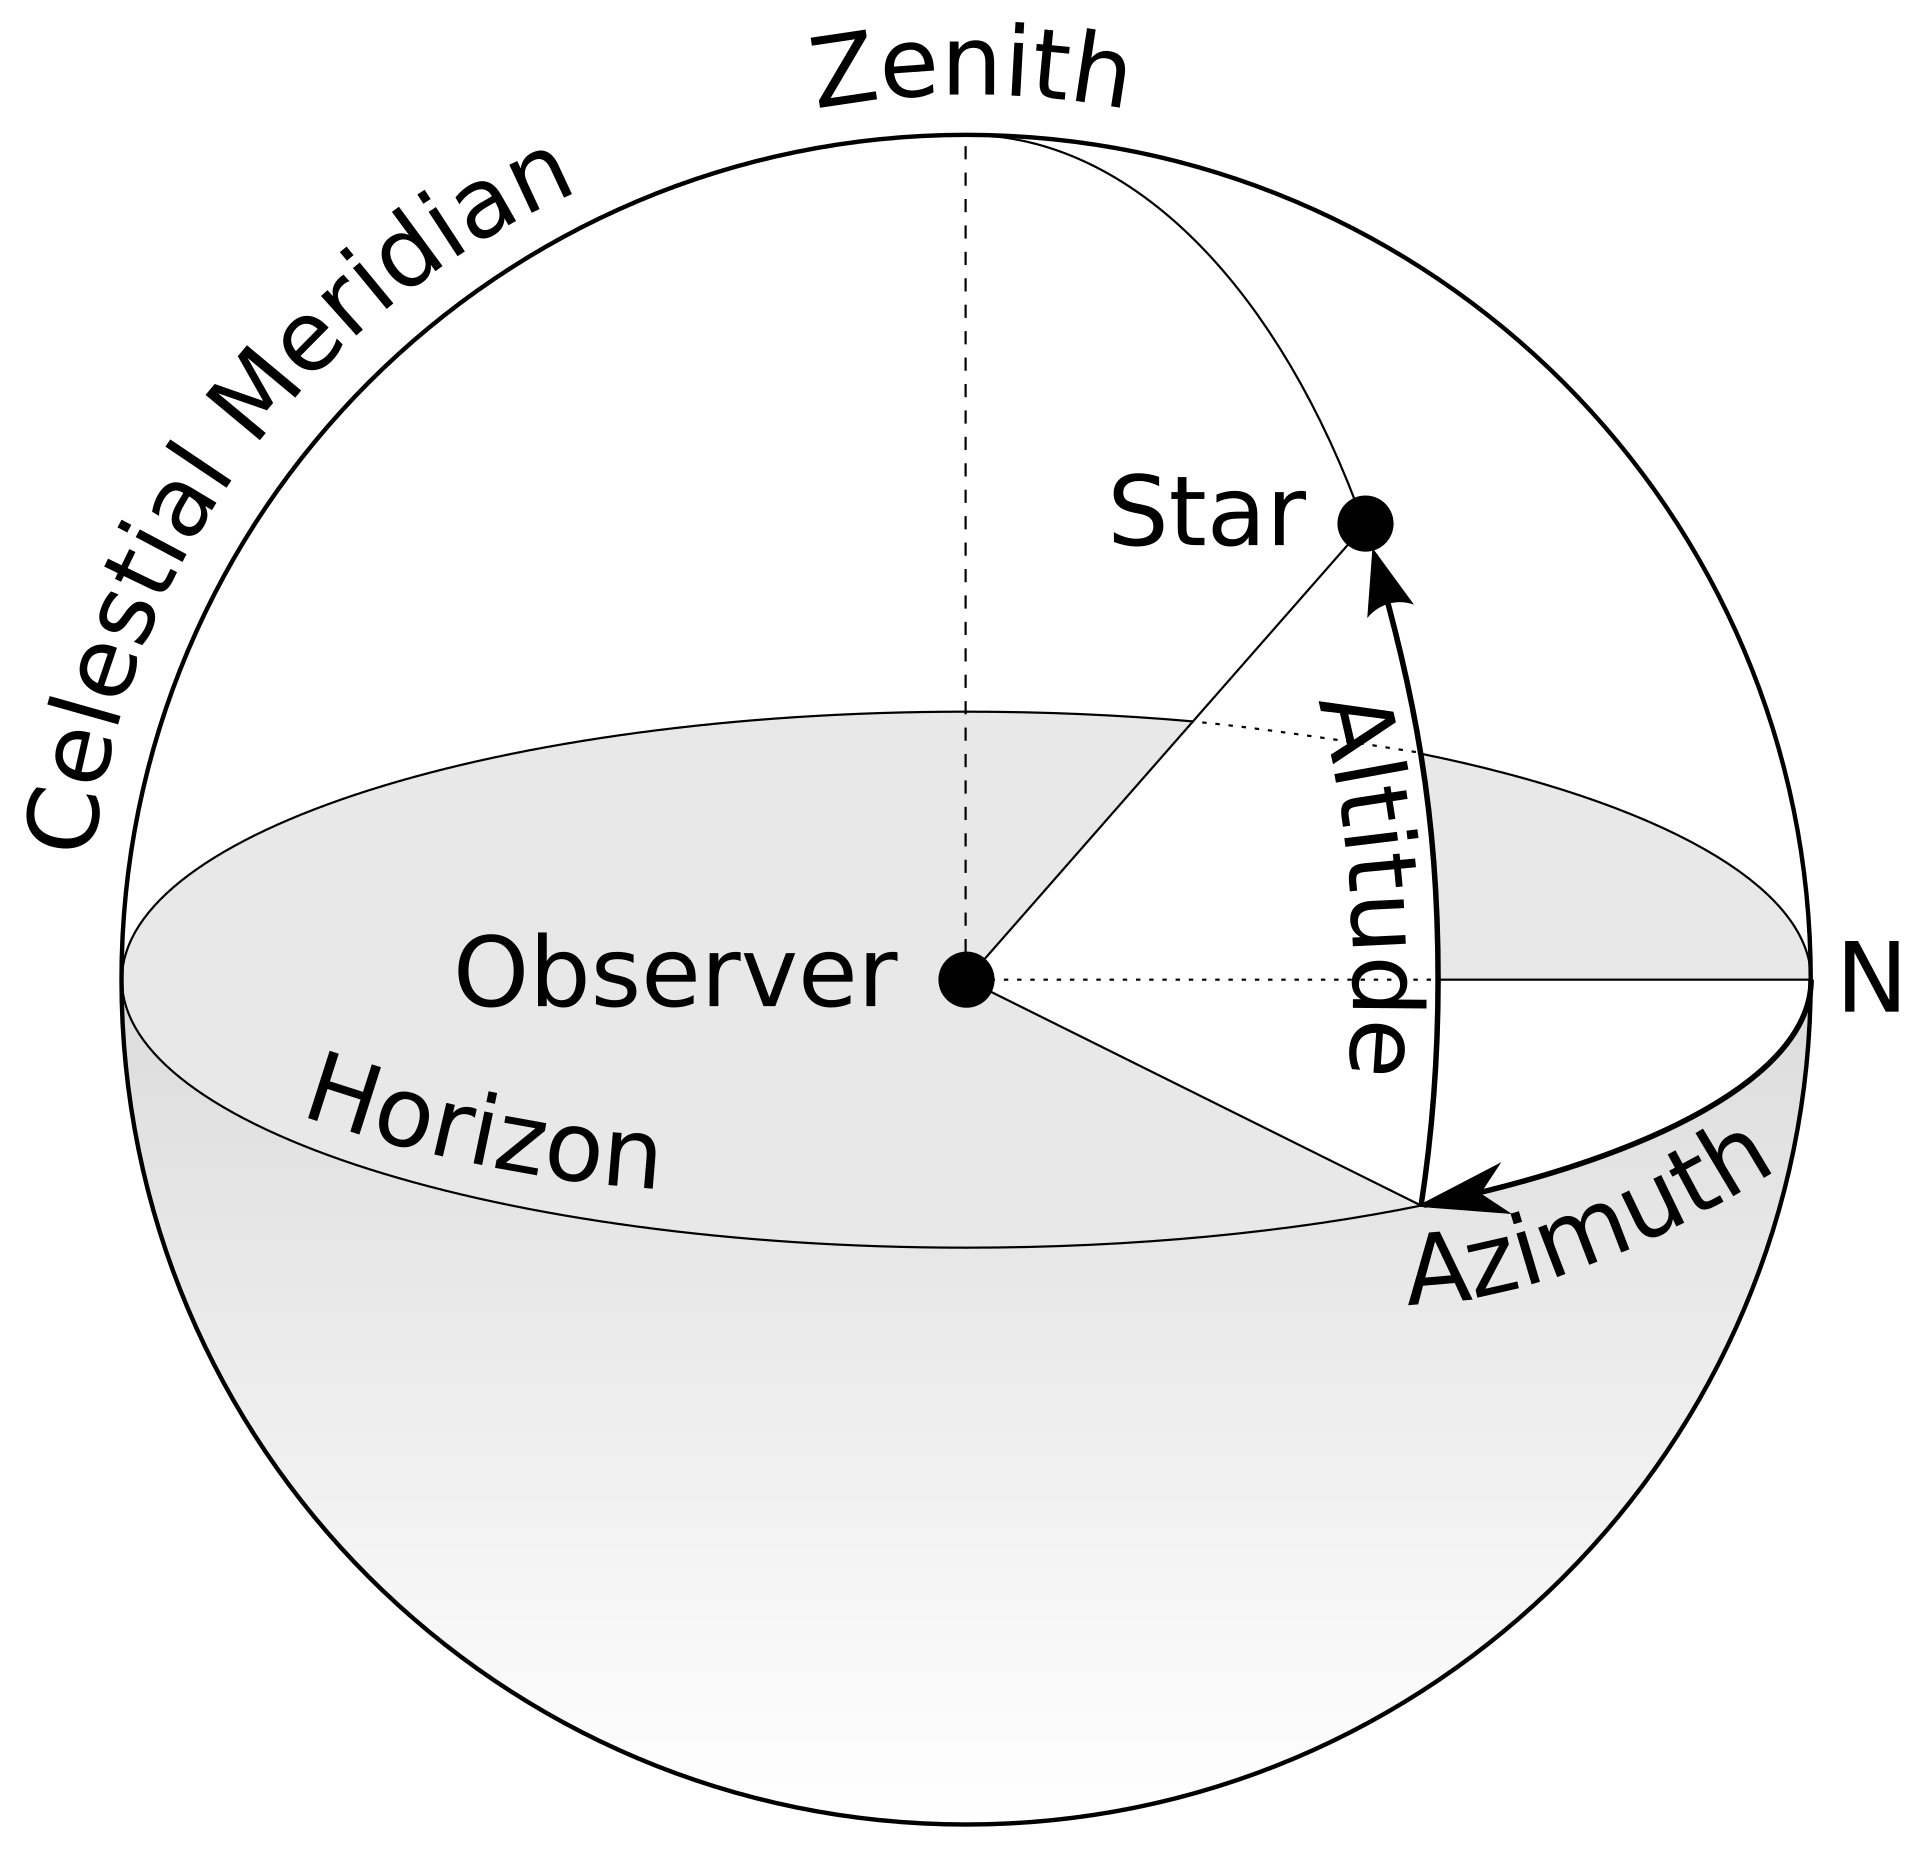
\includegraphics[width=0.6\textwidth]{Astronomy/Azimuth-Altitude_schematic.png}
    \caption[Altitude-azimuth coordinate system]{The altitude-azimuth coordinate system used at APEX. Source \cite{altazschematic}}
    \label{fig:altaz_coords}
\end{figure}




\subsection{Radio/(Sub)-mm Telescope Basics}
In this section, we present an overview of the fundamental components of a radio/(sub)-mm telescope.
As illustrated in subfigure \ref{subfig:radio_telescope}, the basic operation of a Cassegrain single-dish telescope involves collecting electromagnetic radiation with a primary mirror, which is then reflected onto a secondary mirror (subreflector).
The photons are subsequently redirected toward the interior of the telescope, where they are converted into an electrical signal by an attached receiver (instrument).
The electric signal is then processed and recorded for further analysis.

Additionally, subfigure \ref{subfig:beamwidth} provides a visual representation of the telescope's beam.
The telescope's beam indicates the source of the strongest signal detected by the telescope.
The beam power weakens towards the edges, and an object needs to be located within the beam to be observable.
The angular resolution of a telescope, or the solid angle it can observe, is determined by the width of its beam.
Physical characteristics, including the primary dish diameter and the electromagnetic radiation frequency, determine the beam's width.
The standard measure for beamwidth is the half-power beamwidth, or the angle between two points on the beam where the radiation power is half its maximum.

\begin{figure}[H]
    \centering
    \begin{subfigure}[t]{0.49\textwidth}
        \centering
        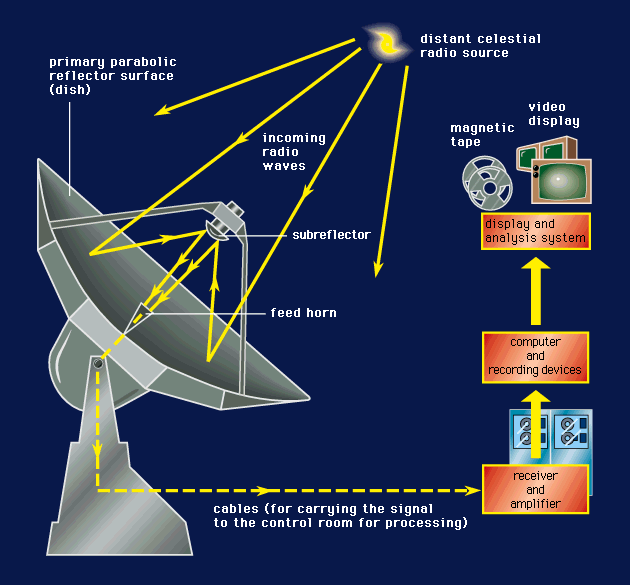
\includegraphics[width=\textwidth]{Astronomy/radio_telescope.png}
        \caption{Radio telescope basics.}
        \label{subfig:radio_telescope}
    \end{subfigure}
    \hfill
    \begin{subfigure}[t]{0.49\textwidth}
       \centering
       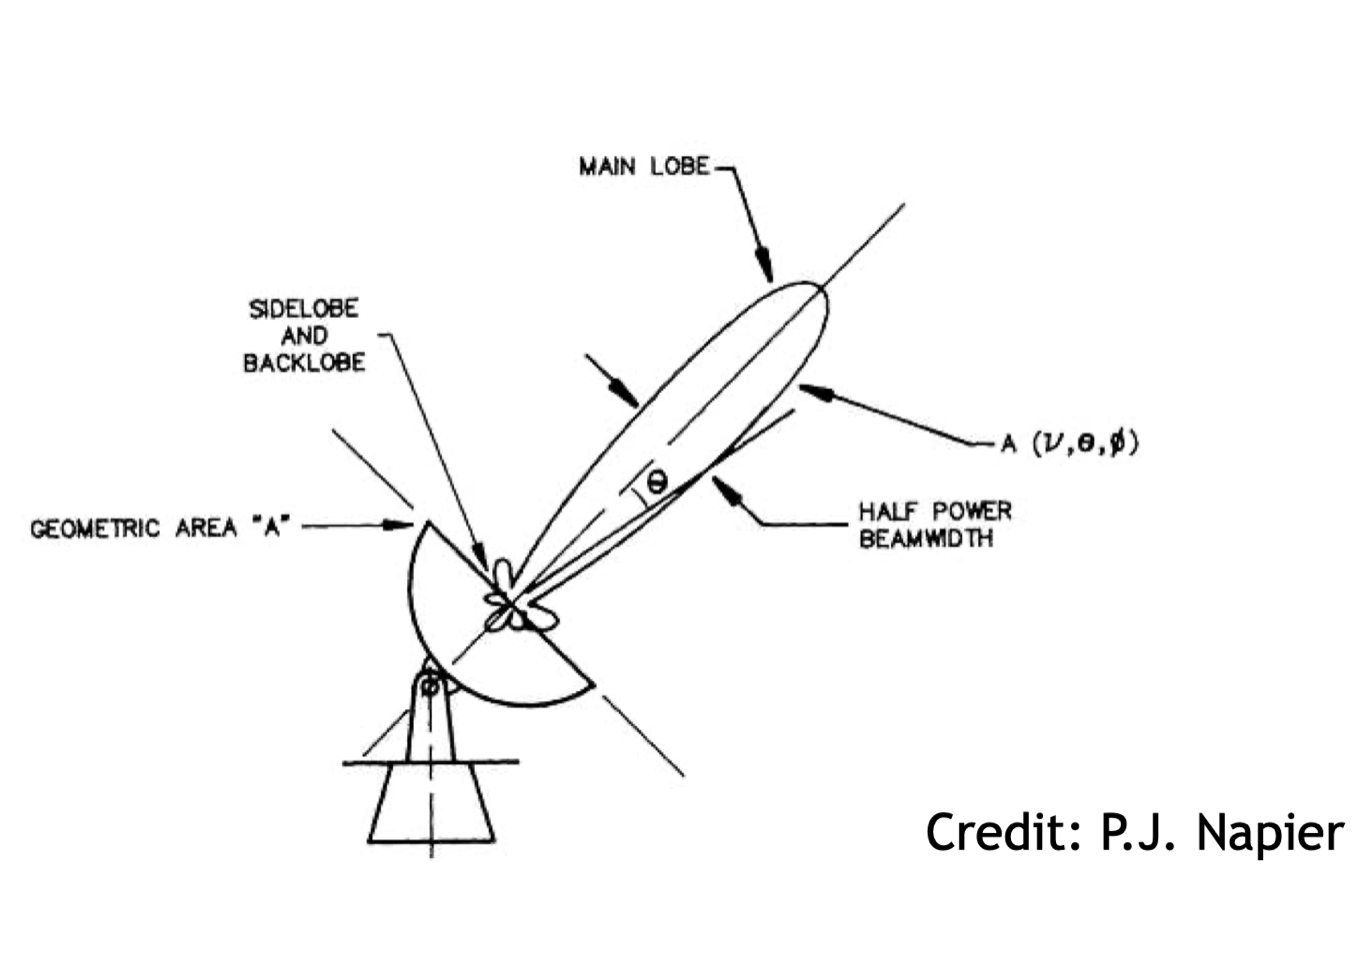
\includegraphics[width=\textwidth]{Astronomy/beamwidth_sketch_cropped.png}
       \caption{Telescope beam sketch.}
       \label{subfig:beamwidth}
    \end{subfigure}
    \caption[Radio telescope basics]{\textbf{a)} Basics of how a radio telescope works and \textbf{b)} Sktech of a telescope's beam.}
    \label{fig:telescope_info}
\end{figure}

% \section{Problem description}
% \textcolor{red}{This section have to be fixed completely}
% A telescope makes high precision observations of objects located very far away from Earth.
% Because of this distance, small changes such as the deformation of mirrors due to temperature might impact the precision drastically.\cc{Claudia Cicone: Here you could explain that astronomical objects are observed as they were "projected" in 2D angular coordinates on the sky, and you could talk about astronomical coordinates (see Lecture 5 notes of my course AST2210 for some explanation and references)
% }
% Over time, these deformations have been observed and analyzed, and in order to counter this, a pointing model is made.
% \cc{Claudia Cicone: The need for a pointing model is relevant mainly to sub-mm telescopes that cannot take real-time images of what they are observing, and so the precision of the pointing direction must be known accurately before starting the observations.}
% The pointing model uses measurements from various instruments and is fitted to the observed offsets.
% The model is used for about a month, or until it start performing poorly.
% The variation in measurements are still too big using only this model, so pointing scans have to be made regularly to correct even more.
% A pointing scan is an observation of an object with known location.
% When doing this, the offset on this observation is then added on top of the pointing model.
% These corrections to azimuth and elevations are used for a couple of hours, until a new pointing scan is made.
% \cc{Claudia Cicone: Need to define azimuth and elevation first, see other comment above
% }
% Using this approach, pointing error is reduced to about $4$ arc seconds.\\

% The aim of this thesis is to investigate the possibility of using machine learning to increase the performance of the telescope, by improving pointing accuracy.
% This can be done in multiple ways.

% One possibility is to apply a pointing model on top of the current pointing model using machine learning, such that the average offset is reduced even more.
% Another possibility is investigating the use of machine learning models to aid such that a pointing scan doesn't have to be made as often.
% This will reduce the workload at the telescope. \\
